Este capítulo aborda o planejamento, análise e execução do método proposto por este trabalho, a fim de verificar a viabilidade do projeto, bem como sua eficiência. O sistema computacional desenvolvido denomina-se \productname{} e tem seu código-fonte disponível em \url{https://github.com/rodrigost23/automailx}.


\section{Planejamento dos experimentos}\label{sec:result_planejamento}

O intuito desta avaliação experimental é verificar a capacidade do sistema \productname{} de classificar as ações do usuário a partir da leitura de sensores, e exibir um modelo virtual animado que demonstra os dados lidos e a detecção dos movimentos realizados. Neste sentido, foram definidas as seguintes questões de pesquisa:

\begin{enumerate}[label=\textbf{QP\arabic*:}, ref=QP\arabic*]
    \item O sistema \productname{} é capaz de replicar os movimentos realizados pelo usuário em um ambiente virtual?\label{qp:simula_movimentos}
    \item O sistema \productname{} pode prever as ações da prótese virtual em tempo real a partir dos dados dos sensores?\label{qp:previsao_sensores}
    \item O sistema \productname{} tem desempenho consistente independente do usuário?\label{qp:usuarios_diferentes}
    \item A acurácia da previsão de movimentos do sistema \productname{} é suficiente para garantir a sua confiabilidade?\label{qp:acuracia}
\end{enumerate}
Visando responder essas questões, foi criado um estudo de caso onde foram testados os seguintes cenários: (1)...\todo{Descrever visando análise cada QP}


\subsection{Captura dos movimentos}\label{sec:result_captura}

O protótipo para captura de dados consiste, um módulo GY\=/\(521\) com um sensor MPU-\(6050\) \cite{invensense:imu_mpu}, que contém um acelerômetro e um giroscópio, e um sensor flexível SparkFun de \(2{,}2\) polegadas~\cite{spectrasymbol:flex_sensor}, conectados em um Arduino Nano conforme o esquema da \autoref{fig:result_schem}.

\begin{figure}[ht]
	\caption{\label{fig:result_schem}Esquema das conexões dos sensores ao Arduino}
	\begin{center}
	    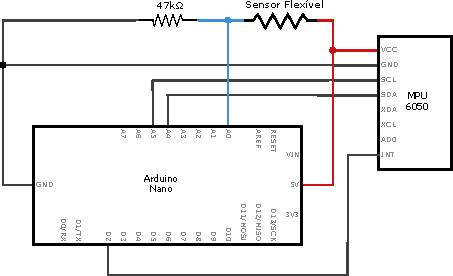
\includegraphics[width=.8\textwidth]{resources/result_schem}
	\end{center}
	\legend{Fonte: Elaborada pelo autor}
\end{figure}

Todos esses equipamentos foram fixados em uma joelheira de material flexível não rígido, como visto na \autoref{fig:result_prototipo}, com o MPU\=/\(6050\) (b) posicionado acima do joelho, e o sensor flexível (a) posicionado na parte de trás. Este último sensor teve de ser posicionado desta forma devido ao seu comprimento de apenas \SI{55.88}{\milli\meter}, já que posicionamento na parte frontal do joelho, como planejado na ~\autoref{sec:metodo_protese}, impediria que a resistência do sensor variasse o suficiente.

\begin{figure}[ht]
	\caption{\label{fig:result_prototipo}Protótipo com o sensor flexível (a) e o MPU-6050 (b) conectados ao Arduino Nano}
    \todo[inline]{Sugiro substituir uma das figuras da joelheira por uma perna usando a joelheira}
	\begin{center}
	    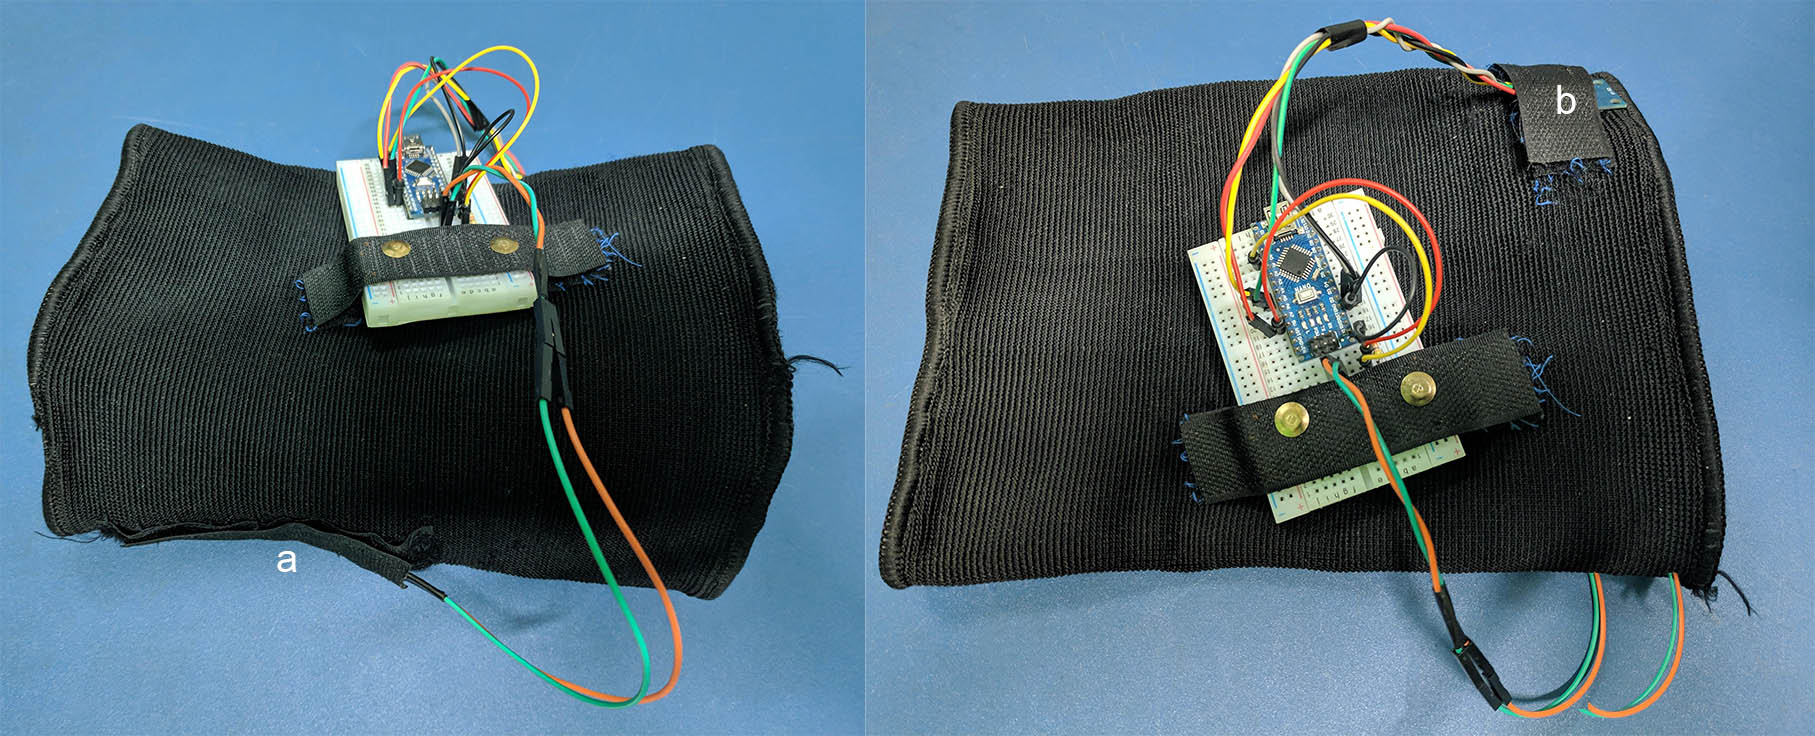
\includegraphics[width=.8\textwidth]{resources/result_prototipo}
	\end{center}
	\legend{Fonte: Elaborada pelo autor}
\end{figure}

Para que fossem feitas a leitura e a classificação dos dados capturados, o Arduino foi conectado via cabo USB em um computador que executava o simulador. Os dados do giroscópio, acelerômetro e resistência do sensor flexível, respectivamente, são enviados continuamente via comunicação serial pelo \textit{software} carregado no Arduino.


\subsection{\textit{Software} de simulação}\label{sec:result_simulacao}

O sistema de simulação é executado em um computador e foi desenvolvido na linguagem Python 3.7, para facilitar o uso da ferramenta scikit-learn. O programa é composto por diversos componentes que se integram para realizar diferentes atividades: leitura dos dados, através da biblioteca \textit{pyserial}\footnote{\url{https://github.com/pyserial/pyserial}}; gravação dos dados em arquivos; classificação dos dados, utilizando scikit-learn; e a exibição 3D com o uso das bibliotecas \textit{PyOpenGL}\footnote{\url{http://pyopengl.sourceforge.net/}} e \textit{pygame}\footnote{\url{https://www.pygame.org/}}.

\section{Execução dos experimentos}\label{sec:result_execucao}

Com o protótipo confeccionado e os \textit{softwares} desenvolvidos, deu-se início à captura de dados dos sensores, na qual observou-se que os melhores dados a serem usados para a classificação dentre os disponíveis seriam os valores do acelerômetro e do sensor flexível, ignorando os dados de orientação do giroscópio, que ainda são utilizados para orientar o modelo virtual.

Foram selecionados indivíduos com os membros intactos para gerar o conjunto de dados que seria utilizado para a classificação. A joelheira foi vestida na perna direita e foi solicitado para que cada um deles caminhasse em linha reta, enquanto era capturado o estado da transição de cada uma das ações.

As ações definidas para este experimento foram apenas voltadas à detecção de uma caminhada plana, classificando cada um dos passos de cada perna. Ou seja, além do estado de repouso (estado 0), foram armazenados o ponto em que a perna esquerda estava para frente (estado 1), e o ponto em que a perna direita estava para frente (estado 2), ilustrados pela \autoref{fig:result_estados}. Ao todo, foram coletadas 140 amostras.

\begin{figure}[ht]
	\caption{\label{fig:result_estados}Demonstração das três ações capturadas para a classificação}
	\begin{center}
	   % 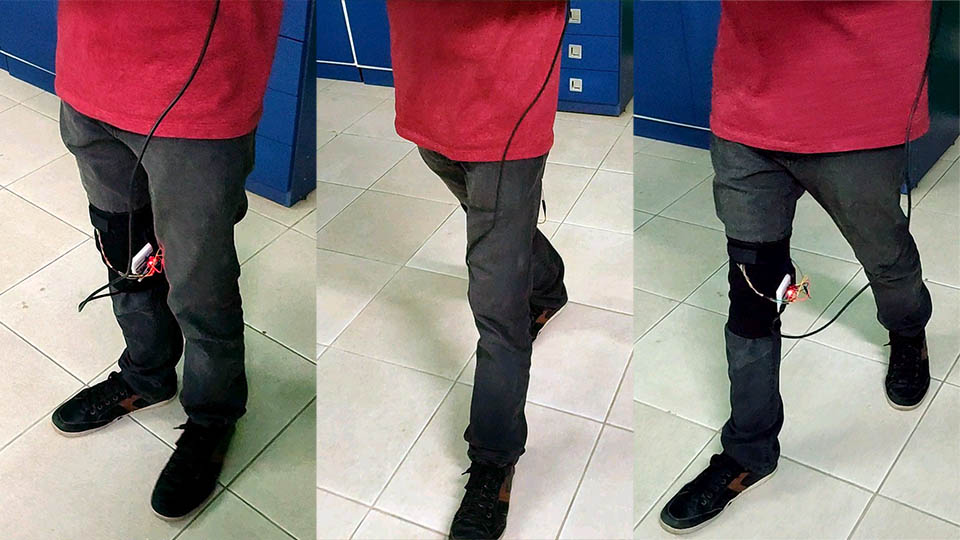
\includegraphics[width=\textwidth]{resources/result_estados}
	   \missingfigure[figwidth=\textwidth, figheight=7cm]{Tirar 3 fotos em cada uma das posições para ilustrar as ações no texto (ou só capturar do vídeo de exemplo)}
	\end{center}
	\legend{Fonte: Elaborada pelo autor}
\end{figure}

A captura foi feita a partir de um cabo USB de \SI{1.5}{\meter} conectado a um \textit{notebook} (com um processador Intel i7\=/7500U, que conta com \textit{clock} de até \SI{3.5}{\giga\hertz}, e \SI{8}{\giga\byte} de RAM) no sistema operacional Manjaro Linux\footnote{\url{http://manjaro.org/}} 18.0.4, estabelecendo comunicação serial com o programa.

\subsection{Análise dos resultados}\label{sec:result_analise}

A partir dos dados coletados dos usuários, verificou-se através de validação cruzada que \textit{Random Forest} seria o algoritmo mais apropriado dentre os disponíveis no scikit-learn, com acurácia de aproximadamente \(82\%\) para os dados combinados de todos os usuários, como pode ser visto no gráfico da \autoref{fig:result_accuracy_rfc}.

\begin{figure}[ht]
	\caption{\label{fig:result_accuracy_rfc}Gráfico de acurácia do algoritmo da Floresta Aleatória para os dados combinados}
% 	\todo[inline]{Tentar gerar um gráfico mais interessante: \url{https://scikit-learn.org/stable/auto_examples/model_selection/plot_cv_indices.html}}
	\begin{center}
	    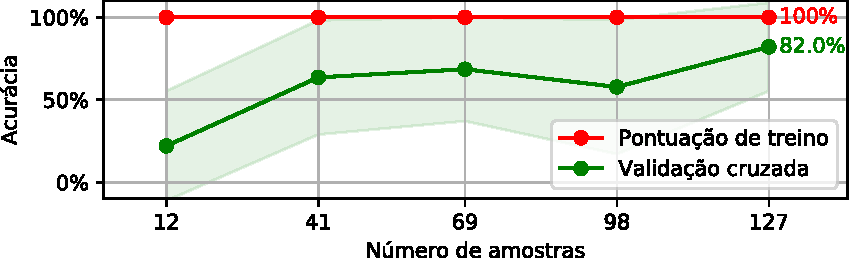
\includegraphics[width=\textwidth]{resources/result_accuracy_rfc}
	\end{center}
	\legend{Fonte: Elaborada pelo autor}
\end{figure}

Ao analisar-se os conjuntos de dados de cada indivíduo, sobressaiu-se a Análise de Discriminantes Lineares (LDA), que obteve aproximadamente \(96{,}9\%\) de acurácia, como demonstra a \autoref{fig:result_accuracy_lda}. Devido ao pequeno número de amostras, não foi possível gerar um conjunto de dados genérico que funcionasse para todos os indivíduos a partir da coleta realizada. Portanto, cada usuário teria que fazer a própria calibragem do dispositivo para prever os próprios movimentos.

\begin{figure}[ht]
	\caption{\label{fig:result_accuracy_lda}Gráfico de acurácia da LDA para um conjunto de dados individual}
% 	\todo[inline]{Tentar gerar um gráfico mais interessante: \url{https://scikit-learn.org/stable/auto_examples/model_selection/plot_cv_indices.html}}
	\begin{center}
	    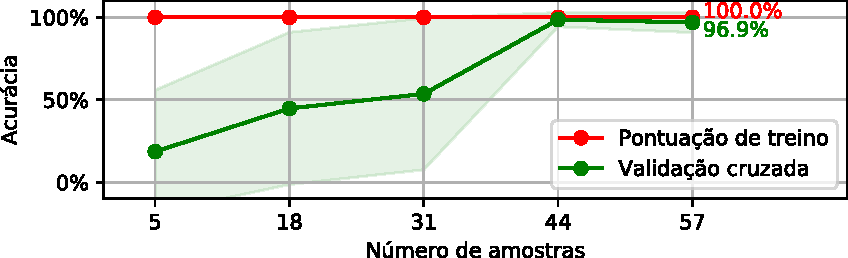
\includegraphics[width=\textwidth]{resources/result_accuracy_lda}
	\end{center}
	\legend{Fonte: Elaborada pelo autor}
\end{figure}


% \begin{figure}[ht]
% 	\caption{\label{fig:result_accuracy_plot}Gráfico de acurácia do algoritmo CART}
% % 	\todo[inline]{Tentar gerar um gráfico mais interessante: \url{https://scikit-learn.org/stable/auto_examples/model_selection/plot_cv_indices.html}}
% 	\begin{center}
% 	    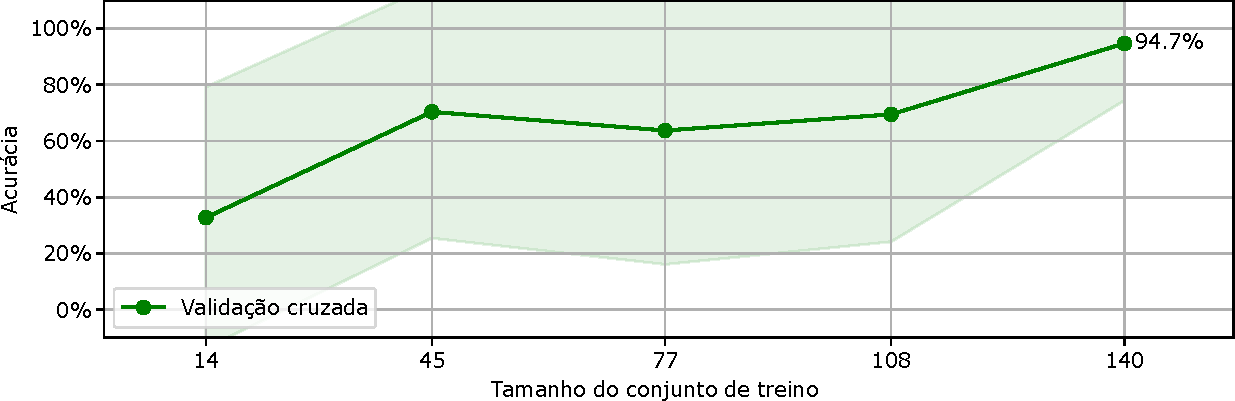
\includegraphics[width=\textwidth]{resources/result_accuracy_plot}
% 	\end{center}
% 	\legend{Fonte: Elaborada pelo autor}
% \end{figure}

A simulação animada em 3D, como vista na~\autoref{fig:result_simulacao} mostrou-se capaz de exibir o movimento realizado pelos dois sensores em tempo real e, com a classificação dos dados, também a ação realizada na prótese simulada, desde que o conjunto de dados utilizado correspondesse apenas aos dados coletados pelo mesmo usuário que estivesse utilizando o dispositivo.

\begin{figure}[ht]
	\caption{\label{fig:result_simulacao}Visualização da posição da perna do usuário e simulação da prótese}
	\begin{center}
	    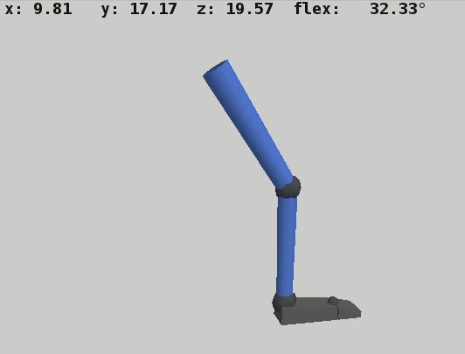
\includegraphics[width=.8\textwidth]{resources/result_simulacao}
	\end{center}
	\legend{Fonte: Elaborada pelo autor}
\end{figure}

Algumas limitações em relação aos sensores selecionados foram observadas: a falta de um magnetômetro no MPU\=/6050 utilizado impede que ele estabeleça uma orientação realista em relação ao mundo real, fazendo com que a simulação não reconhecesse bem movimentos de virada. Além disso, ao longo dos experimentos realizados, notou-se que o sensor flexível ficou cada vez menos preciso, o que tornou a visualização 3D um pouco menos realista, pois o ruído nos dados do sensor tornou-se maior, mas não impediu que os dados fossem classificados e as ações previstas.